

\chapter{实验结果及分析}

\section{手工测试}
我们将 liso\_client 设置为忙等待,及其不会自动关闭 socket 并退出,而是占用着服务器的资源等待着。如图\ref{fig:lab4test1},我们同时开启了 4 个陷入忙等待的客户端对服务器发出请求,服务器仍然能正常处理发出 pipeline 请求的客户端。


\begin{figure}[htbp!]
    \centering 
    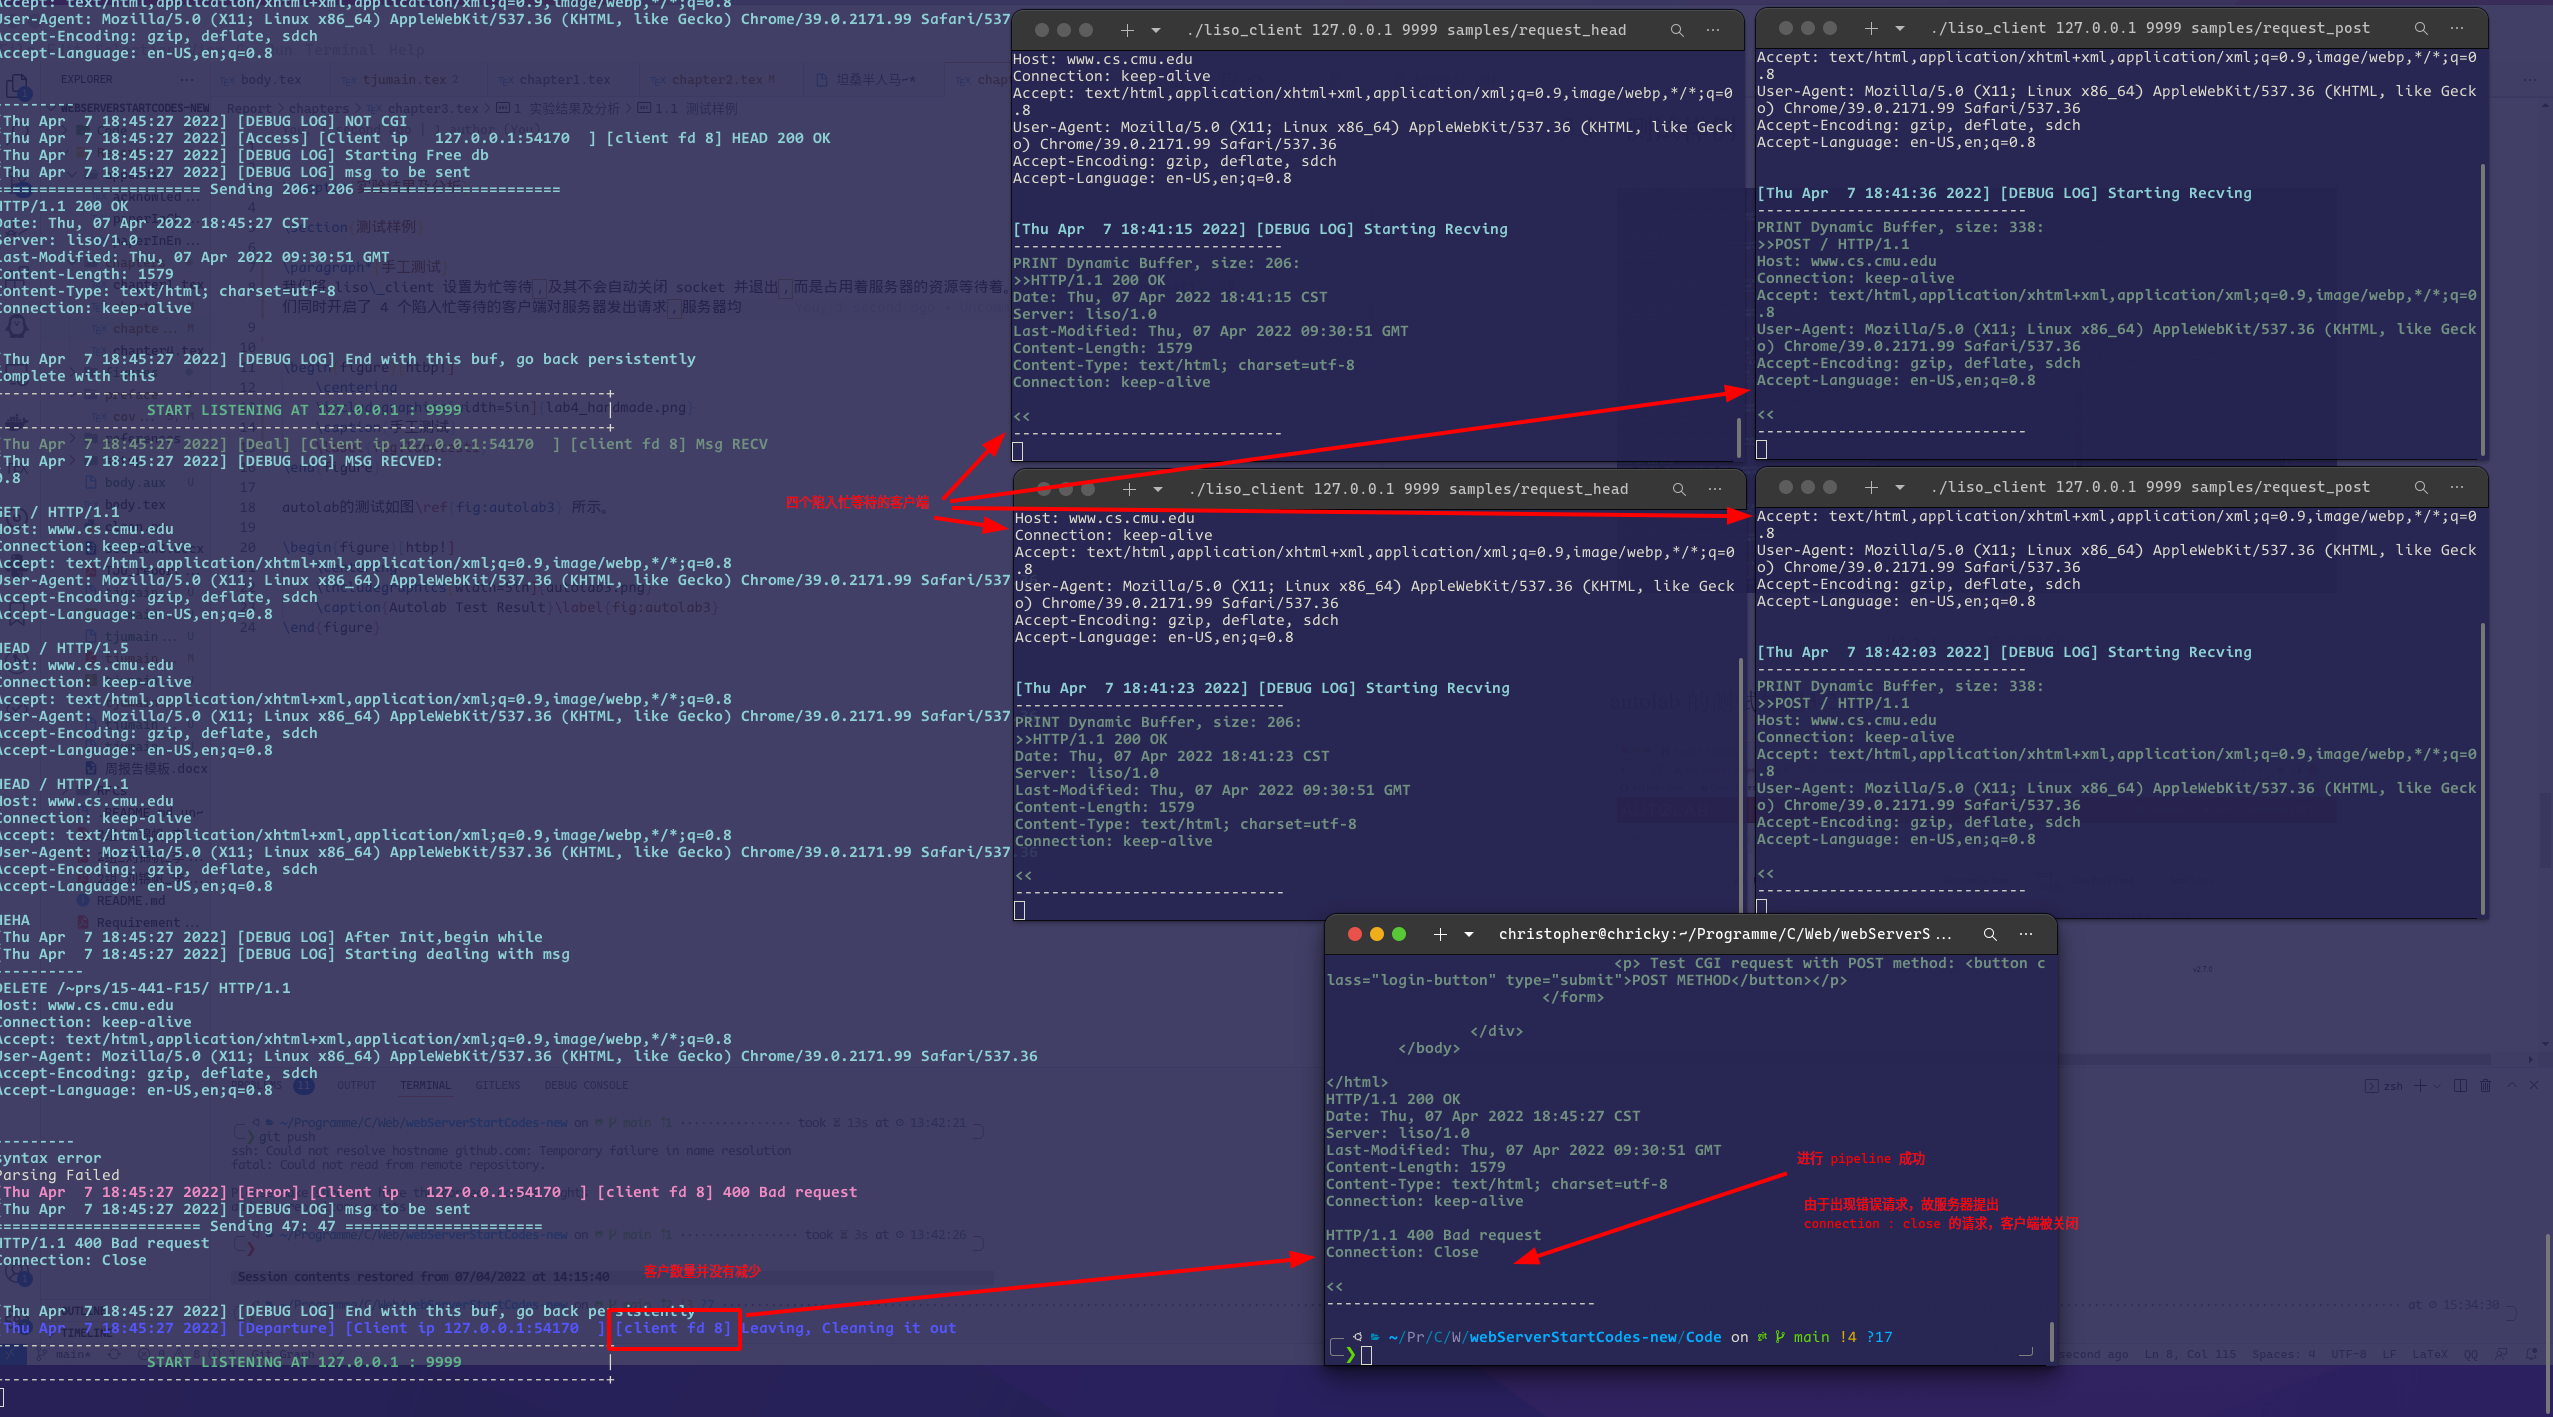
\includegraphics[width=6in]{lab4_handmade.png}
    \caption{手工测试}
    \label{fig:lab4test1}
\end{figure}

\section{Autolab 测试} 如图\ref{fig:autolab4} 所示,在 3月29日 下午完成了基础功能,后续修改了部分细节(同时也在进行 CGI 的编程)。

\begin{figure}[htbp!]
    \centering
    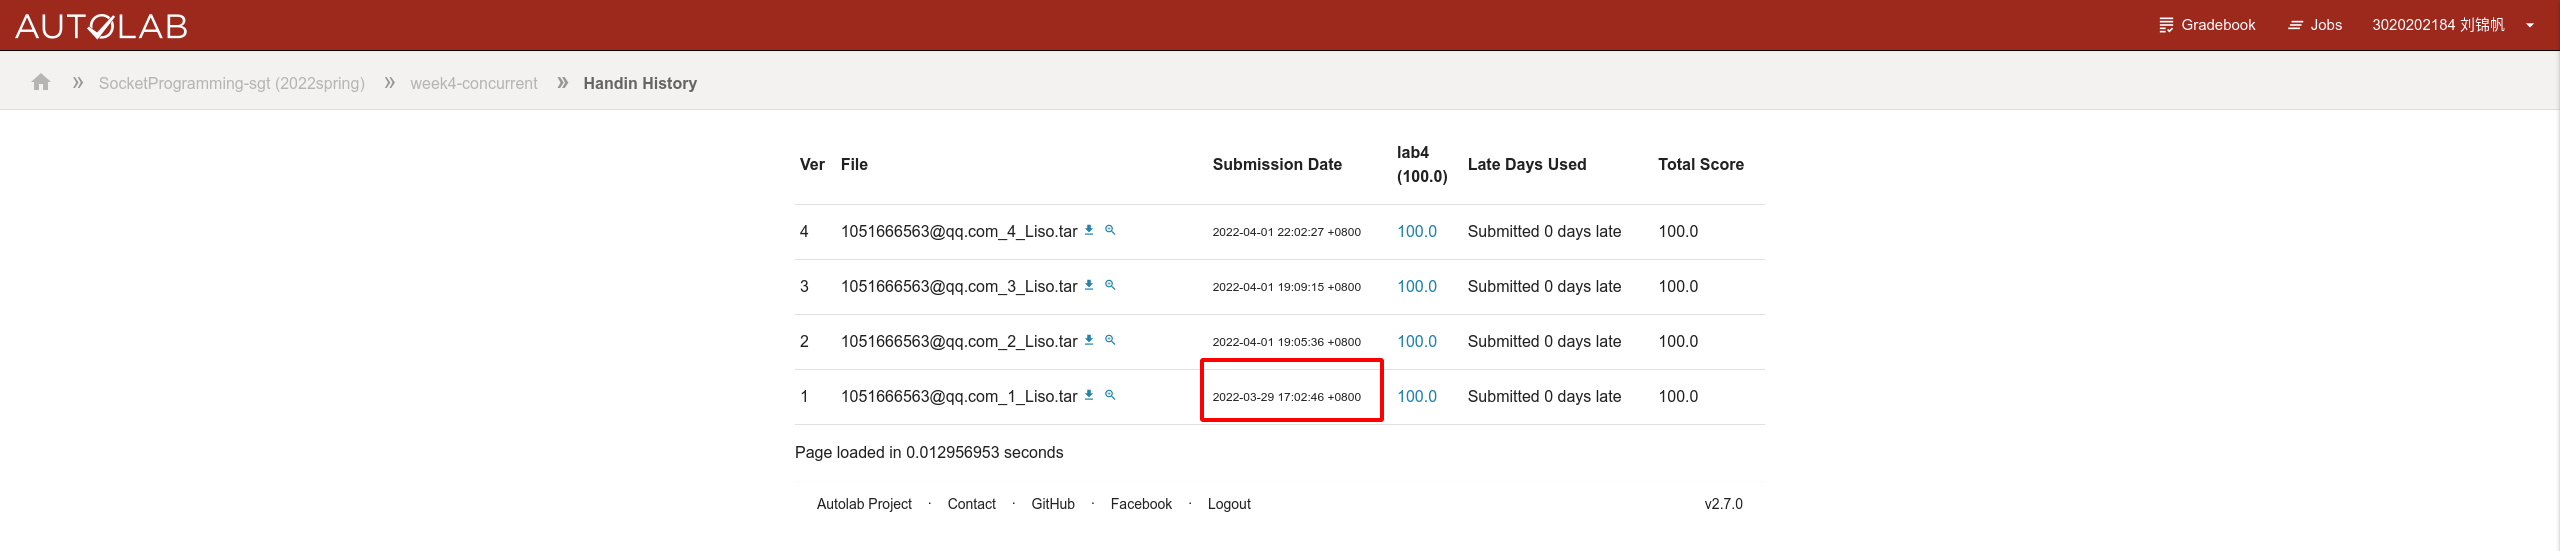
\includegraphics[width=6in]{autolab4.png}
    \caption{Autolab Test Result}\label{fig:autolab4}
\end{figure}

\section{Apache 测试} 
我们分别进行了并发压力测试以及多请求压力测试。测试截图统一放在附录中。
第三周的 liso\_server 由于没有进行并发优化。在测试时由于会一直等待客户端提出退出申请,在测试时会出现 Apache Bench 忙等待。故而我们只对第四周的 liso\_server 进行了测试。

\paragraph*{并发压力测试} 控制总请求数不变的情况下,我们分别进行了并发数量为 10、100 以及 1000 的测试,结果如图所示。如表\ref{tab:parallel} 所示,总请求数量不变情况下,随着并发等级的提高,单个请求的平均反应时间并没有太大的变化。所以可以认为我们的方案是能够解决高并发问题的。

\begin{table}[htbp!]
    \centering
    \begin{tabular}{llll}\hline
      & 并发等级 & 总请求数量 & TPR(ms)   \\\hline
    1 & 10   & 1000  & 0.238 \\
    2 & 100  & 1000  & 0.247 \\
    3 & 1000 & 1000  & 0.222\\
    \hline
    \end{tabular}
    \caption{并发压力测试结果}\label{tab:parallel}
\end{table}

\paragraph*{多请求压力测试} 通过控制并发等级为10不变,改变总请求数量,我们得到了多请求压力测试的结果,如表\ref{tab:multiple}所示。可以轻易看出,在并发等级一定的情况下,总请求数量在100,000量级及以下时,单个请求的平均反应时间都能在正常的范围中。但当请求量达到1,000,000 数量级时,单个请求的平均相应时间则会增加很多,推测是因为请求数量太多,导致频繁接受、删除用户,进而导致反应时间增加。

\begin{table}[htbp!]
    \centering
    \begin{tabular}{llll}\hline
      & 并发等级 & 总请求数量 & TPR(ms)   \\\hline
    1 & 10      & 100       & 0.332 \\
    2 & 10      & 1000      & 0.238 \\
    3 & 10      & 10000     & 0.225\\
    4 & 10      & 100000    & 0.264\\
    5 & 10      & 1000000   & 0.463\\
    \hline
    \end{tabular}
    \caption{多请求压力测试}\label{tab:multiple}
\end{table}
